\begin{englishtitle}
\title{Planar Flows with Minimal Ratio of the Extremal
Values of the Pressure on the Free Boundary\thanks{Работа выполнена при поддержке РФФИ, 
грант \textnumero~20-01-00469.}}
% First author
\author{Alexandre Demidov}
\institute{MSU, Moscow, Russia\\
  {demidov.alexandre@gmail.com}}
% etc

\maketitle

\begin{abstract}
Necessary conditions are given, as well as sufficient conditions 
for the existence of a free boundary, under which the minimum ratio 
of extremal values for  the modules of the gradient of a harmonic 
function of a given class is achieved. Calculation formulas are received. 


\keywords{flat currents, minimum ratio, extreme values on free boundary}
\end{abstract}
\end{englishtitle}



\iffalse

\documentclass[12pt]{llncs}
\usepackage[T2A]{fontenc}
\usepackage[utf8]{inputenc}
\usepackage[english,russian]{babel}
\usepackage[russian]{nla}
\usepackage{graphicx}


\newcommand{\R}{\mathbb{R}}
\newcommand{\mC}{\mathbb{C}}
%\newcommand{\C}{\mathbb{C}}
\newcommand{\T}{\mathbb{T}}
\newcommand{\V}{\mathbb{V}}
\newcommand{\bH}{\mathbf{H}}
\newcommand{\bI}{\mathbf{I}}
\newcommand{\bK}{\mathbf{K}}
\newcommand{\bF}{\mathbf{F}}
\newcommand{\bk}{\mathbf{k}}
\newcommand{\bff}{\mathbf{f}}
\newcommand{\bR}{\mathbf{R}}
\newcommand{\bS}{\mathbf{S}}
\newcommand{\bT}{\mathbf{T}}
\newcommand{\br}{\mathbf{r}}
\newcommand{\bs}{\mathbf{s}}
\newcommand{\bg}{\mathbf{g}}
%\newcommand{\G}{\mathbb{G}}
\newcommand{\Z}{\mathbb{Z}}
\newcommand{\N}{\mathbb{N}}
\newcommand{\fD}{\mathfrak{D}}
\newcommand{\fE}{\mathfrak{E}}
\newcommand{\fj}{\mathfrak{j}}
\newcommand{\cN}{\mathcal{N}}
\newcommand{\fM}{\mathfrak{M}}
\newcommand{\fN}{\mathfrak{N}}
%\newcommand{\fD}{\mathfrak{D}}
\newcommand{\fA}{\mathfrak{A}}
\newcommand{\fB}{\mathfrak{B}}
%\newcommand{\fM}{\mathfrak{M}}
\newcommand{\fF}{\mathfrak{F}}
\newcommand{\fH}{\mathfrak{H}}
\newcommand{\fG}{\mathfrak{G}}
\newcommand{\fS}{\mathfrak{S}}
\newcommand{\fQ}{\mathfrak{Q}}
%\newcommand{\x}{{\mathbf x}}
\newcommand{\be}{{\beta}}
%\newcommand{\hi}{{\varphi}}
%\newcommand{\V}{{\overrightarrow V}}
\newcommand{\x}{{\mathbf x}}
\newcommand{\hi}{{\varphi}}
%\newcommand{\be}{{\beta}}
%\newcommand{\V}{{\overrightarrow V}}
\newcommand{\sgn}{\mathop{\rm sgn}\nolimits}
\newcommand{\Var}{\mathop{\rm Var}\nolimits}
\newcommand{\sih}{\mathop{\rm sh}\nolimits}
\newcommand{\coh}{\mathop{\rm ch}\nolimits}
\newcommand{\tah}{\mathop{\rm th}\nolimits}
\newcommand{\cotah}{\mathop{\rm cth}\nolimits}
\newcommand{\atg}{\mathop{\rm arctg}\nolimits}
\newcommand{\actg}{\mathop{\rm arcctg}\nolimits}
%\newcommand{\tg}{\mathop{\rm tg}\nolimits}
%\newcommand{\ctg}{\mathop{\rm ctg}\nolimits}
\newcommand\gA{\mathfrak A}
\newcommand\cA{\mathcal A}
\newcommand\cB{\mathcal B}
\newcommand\gD{\mathfrak D}
\newcommand\cC{\mathcal C}
\newcommand\cD{\mathcal D}
\newcommand\cE{\mathcal E}
\newcommand\cF{\mathcal F}
\newcommand\cI{\mathcal I}
\newcommand\cK{\mathcal K}
\newcommand\cL{\mathcal L}
\newcommand\cM{\mathfrak M}
\newcommand\cR{\mathcal R}
\newcommand\cT{\mathcal T}
\newcommand\cQ{\mathcal Q}
\newcommand\cU{\mathfrak U}
\newcommand\cV{\mathfrak V}
\newcommand\bbH{\mathbb H}
\newcommand\bbN{\mathbb N}
\newcommand\bbI{\mathbb I}
\newcommand\bbK{\mathbb K}
\newcommand\bbF{\mathbb F}
\newcommand\bbC{\mathbb C}
\newcommand\bbR{\mathbb R}
\newcommand\bbZ{\mathbb Z}
\newcommand\mbs{\mathbf s}
\newcommand\bnu{{\boldsymbol \nu}}
\newcommand\bpsi{{\boldsymbol \psi}}
\newcommand\bchi{{\boldsymbol \chi}}
\newcommand\btau{{\boldsymbol \tau}}
\newcommand\brho{{\boldsymbol \rho}}
\newcommand\bfr{{\boldsymbol r}}
\newcommand\bflam{{\boldsymbol \lambda}}
\newcommand\bfsig{{\boldsymbol \sigma}}
\newcommand\bfa{{\boldsymbol a}}
\newcommand\bfbet{{\boldsymbol \beta}}
\newcommand{\pd}[2]{\frac{\partial #1}{\partial #2}}
\newcommand{\p}{\partial }
\newcommand{\eps}{\varepsilon }
\newcommand{\vhi}{\varphi }

\newcommand{\DD}[2]{\frac{\partial {#1}}{\partial {#2}}}
\newcommand{\bE}{\begin{equation}}
\newcommand{\eE}{\end{equation}}
\newcommand{\bEs}{\begin{equation*}}
\newcommand{\eEs}{\end{equation*}}
\newcommand{\bEa}{\begin{eqnarray}}
\newcommand{\eEa}{\end{eqnarray}}
\newcommand{\bEau}{\begin{eqnarray*}}
\newcommand{\eEau}{\end{eqnarray*}}
\newcommand{\bEu}{\begin{displaymath}}
\newcommand{\eEu}{\end{displaymath}}
\newcommand{\gae}{\stackrel{_>}{\sim}}
\newcommand{\lae}{\stackrel{_<}{\sim}}
\newcommand{\DL}{\left}
\newcommand{\DR}{\right}


\newcommand\const{\operatorname{const}}
\raggedbottom

\DeclareMathOperator{\arccot}{arccot}
\DeclareMathOperator{\supp}{supp}

\newtheorem{prop}{Предложение}%[section]
\newtheorem{lem}{Лемма}%[section]
%\newtheorem{theorem}{Theorem}[section]
%\newtheorem{theorem}{Теорема}%[section]
%\newtheorem{problem}{Задача}[section]
%\newtheorem{definition}{Определение}[section]
\newtheorem{cor}{Следствие}%[section]
\newtheorem{aff}{Affirmation}%[section]
%\newtheorem{remark}{Замечание}%[section]
%\newtheorem{proof}{Доказательство}%[section]

%\renewcommand\thesection{\Roman{section}}


%%%%%%%%%%%%%%%%
%\renewcommand\thesection{\Roman{section}}

\makeatletter
\renewcommand\section{\@startsection {section}{1}{\z@}%
                                   {-3.5ex \@plus -1ex \@minus -.2ex}%
                                   {2.3ex \@plus.2ex}%
                                   {\MakeUppercase\normalfont\large\bfseries\sffamily\S~}}
\long\def\@makecaption#1#2{%
  \vskip\abovecaptionskip
  \sbox\@tempboxa{#1. #2}%
  \ifdim \wd\@tempboxa >\hsize
    #1. #2\par
  \else
    \global \@minipagefalse
    \hb@xt@\hsize{\hfil\box\@tempboxa\hfil}%
  \fi
 \vskip\belowcaptionskip}
\makeatother

\fi

%%%%%%%%%%%%%%%%%%%%%%%%%%%%%%%%%%%%%%%%%%%%%








\iffalse
%%%%%%%%%%%%%%%%%%%%%%%%%%%%%%%%%%%%%%%%%%%

%\usepackage[english,russian]{nla}

% \graphicspath{{pics/}} %Set the subfolder with figures (png, pdf).

%\usepackage{showframe}
\begin{document}
%\selectlanguage{russian}
\fi


\title{Плоские течения с минимальным отношением экстремальных значений давления\\ на свободной границе
}
% Первый автор
\author{А.~С.~Демидов 
  %\and
% Второй автор
 % И.~О.~Фамилия\inst{2}
 % \and
% Третий автор
 % И.~О.~Фамилия\inst{2}
} % обязательное поле
\institute{Мехмат МГУ, Москва, Россия\\
  {demidov.alexandre@gmail.com}
  %\and
%Институт (название в краткой форме), Город, Страна\\
%\email{email}
}
% Другие авторы...

\maketitle

\begin{abstract}
Даны необходимые, а также достаточные условия существования свободной границы, 
на которой достигается минимум отношения экстремальных значений модуля градиента 
гармонической функции заданного класса. Получены расчетные формулы.

\keywords{плоские течения, минимум отношения экстремальных значений на 
свободной границе}
\end{abstract}

{\bf 1.} В области $\Omega=\Omega_{\gamma}\subset\mathbb{R}^2$ с искомой (свободной) 
границей ${\gamma}$ класса $C^{k+1,\lambda}$ (целое $k\ge 0$ и $\lambda\in(0,1)$
фиксированы) рассматривается задача на минимум
\begin{equation}
 \label{MINIM}
\Phi(\gamma)=\left.\max_{P\in \gamma}\left|\frac{\partial u}{\partial\nu}
(P)\right|\right/ \min_{P\in \gamma}\left|\frac{\partial u}{\partial\nu}
(P)\right|\; \to\;\inf
\end{equation}
отношения экстремальных значений на~${\gamma}$ модуля градиента гармонической 
функции $u$. 

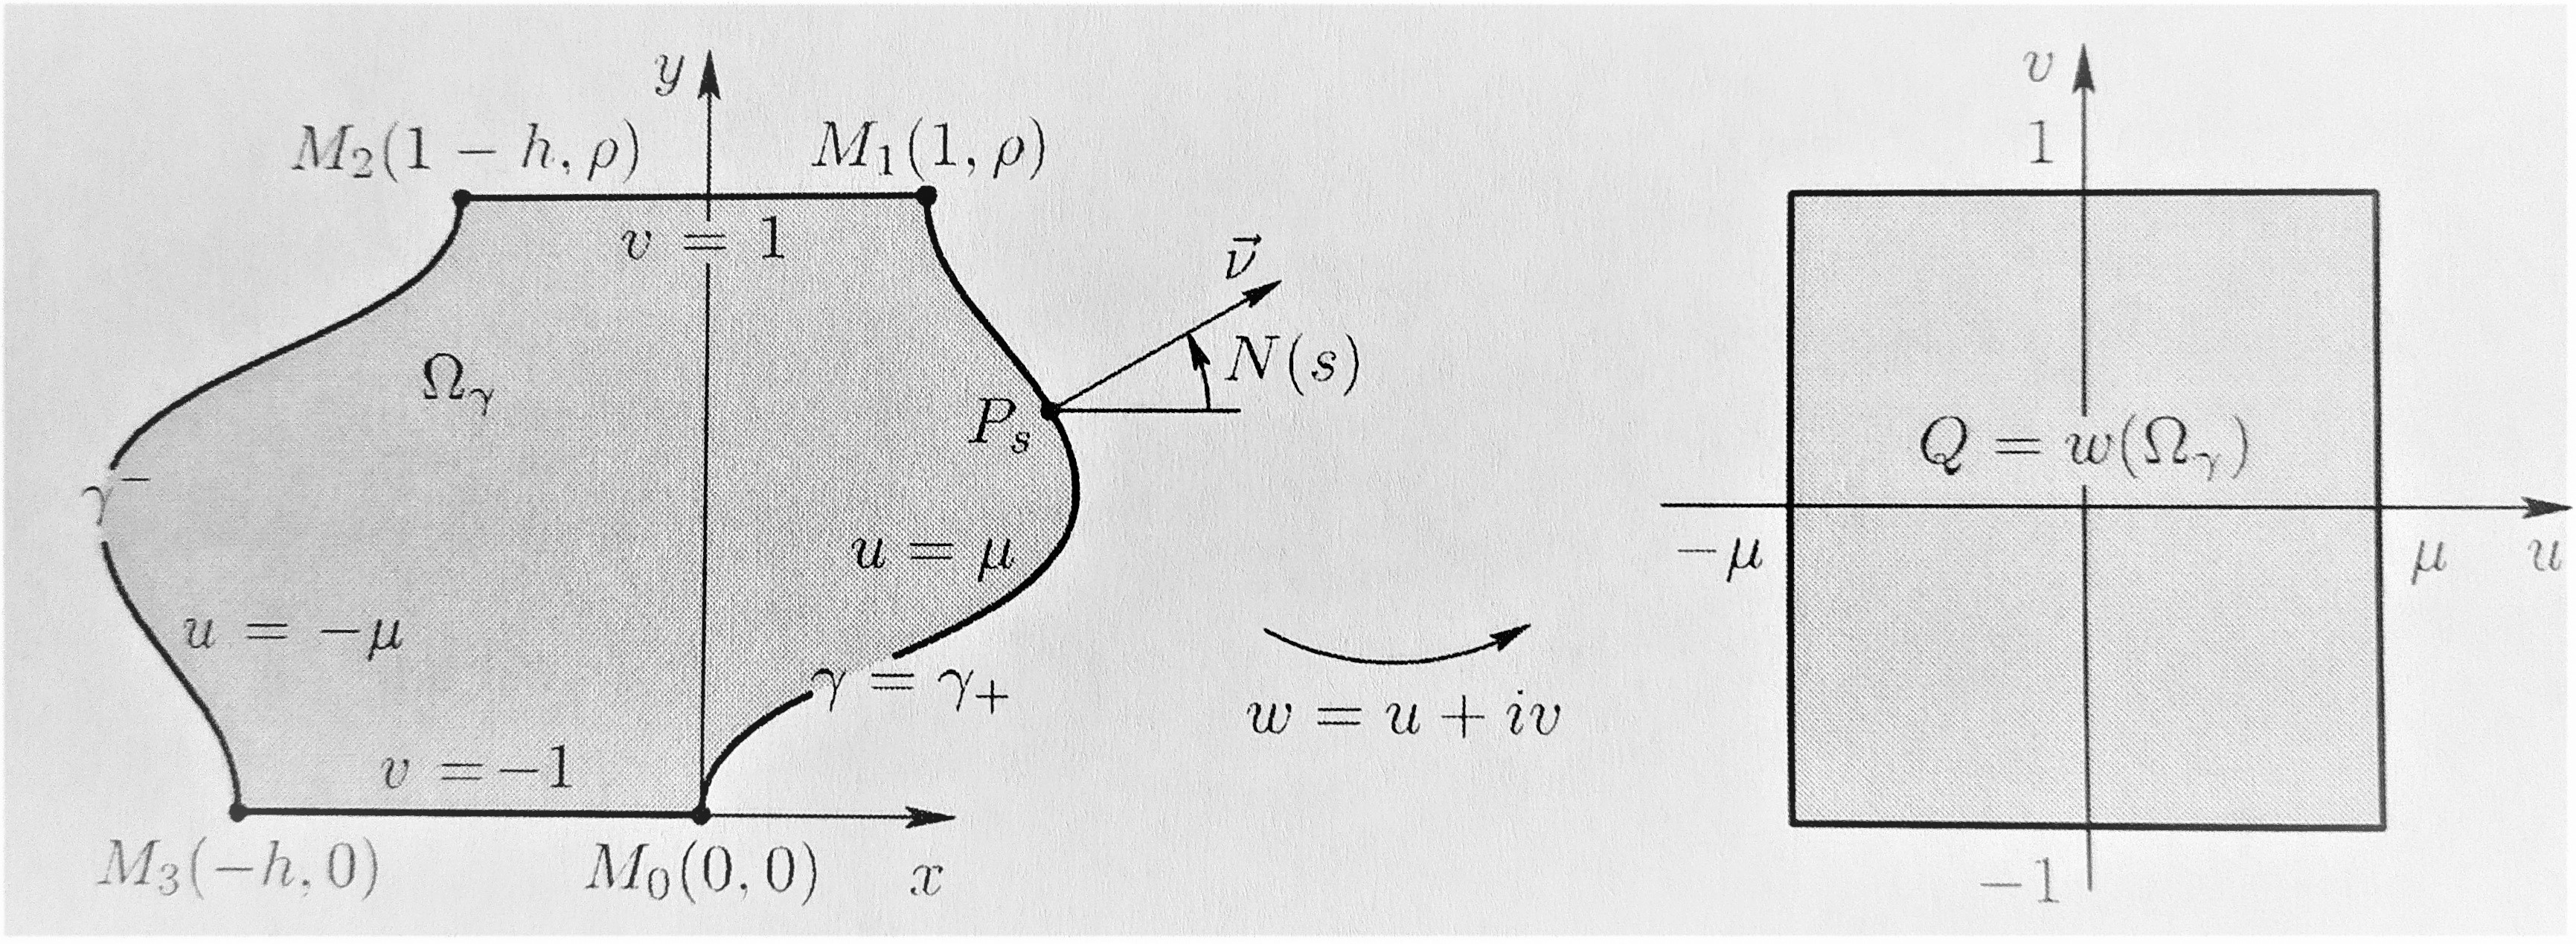
\includegraphics[width=16cm]{Demidov_picture_graph_2}

Функция $w=u+iv$ однолистно отображает односвязную
центрально-симметричную область 
$\Omega=\Omega_{\gamma}\subset\mathbb{C}$
на прямоугольник $Q=\{|u|<\mu, \;|v|<1\}$ и при этом
\begin{equation*}
\label{extr6.1}
 u=\pm \mu \quad \mbox{на}\; \gamma_\pm, \qquad  v=-1
\quad \mbox{на}\; M_3M_0\quad \mbox{и}  \quad v=1 \quad
\mbox{на}\; M_1M_2 \,.
\end{equation*}
Здесь $\mu$~--- заданное число, область
$\Omega_{\gamma}$ ограничена отрезками $M_{3}M_{0}\, , M_{1}M_{2}$
и центрально-симметричными кривыми $\gamma=\gamma_{_+}$ и $\gamma_{_-}$, а 
функция $N(s)$ есть угол между осью $x$ и нормалью к кривой $\gamma$ в 
точке~$P_s\in \gamma$, отстоящей вдоль $\gamma$ на расстоянии $s$ от точки $M_0$.

Пусть 
\begin{equation}
\label{e8}  \beta(v) = N(s(v)), \quad
 s : \left[-1,1\right]\ni v\mapsto s(v) = \int_{-1}^v e^{\alpha(\eta)}\, d\eta,\quad
 \alpha(v)=A(\mu,v),
\end{equation}
где $A+iB$ аналитическая в $Q$, а функция $B$ такова, что $\Delta B = 0$
в $Q$, $B(u,\pm 1)=0$, $B(\pm \mu,v)=\beta(\pm v)$. 
Рассмотрим кривую
\begin{equation}
\label{zmu}
 z(\mu,\cdot ): \, \left[-1,1\right]\ni v \mapsto z(\mu,v)=
i \int_{-1}^v
\exp\left[{\alpha}(\eta)+i{\beta}(\eta)\right]\,d\eta\,,
\end{equation}
где $z: Q\ni w=u+iv \mapsto z(w)=\int_{\mu-i}^w \exp \left[
A(u,v)+iB(u,v) \right]$.
\begin{lemma}
Пусть $F_1(\alpha,\beta){=}\rho - \int\limits_{-1}^1 e^{\alpha(v)}
\cos\beta(v)\,dv$, $F_2(\alpha,\beta){=}1+
\int\limits_{-1}^1 e^{\alpha(v)} \sin\beta(v)\,dv$,
а $\rho$ есть ордината точки $M_1(1,\rho)$ (см. рисунок). Пусть
$z(w)=\int_{\mu-i}^w \exp \left[ A(u,v)+iB(u,v) \right]$, где $w=u+iv\in Q$. 
Тогда кривая
\begin{equation}
\label{zmu}
 z(\mu,\cdot ): \, \left[-1,1\right]\ni v \mapsto z(\mu,v)=
i \int_{-1}^v
\exp\left[{\alpha}(\eta)+i{\beta}(\eta)\right]\,d\eta\,,
\end{equation}
принадлежит классу допустимых кривых,
если и только если 
 $F_1(\alpha,\beta)=0,$ $F_2(\alpha,\beta)=0.$
\end{lemma}

Обозначим через
$\widehat{\alpha}$ и $\widehat{\beta}$ те функции $\alpha$ и
$\beta$, определенные формулами \eqref{e8}, которым соответствуют
кривая $\widehat{\gamma},$ на которой
достигается минимум функционала~\eqref{MINIM}. 
\begin{theorem}
Функции $\widehat{\alpha}$ и $\widehat{\beta}$ дают решение задачи
\begin{equation}
\label{e11} F_0(\alpha)\to \inf,\qquad F_1(\alpha,\beta)=0,\qquad
F_2(\alpha,\beta)=0,
\end{equation}
где $ F_0(\alpha)= \alpha^+ - \alpha^-$, $\alpha^+ = \max_{|v|\le 1}\alpha(v)$,
$\alpha^- = \min_{|v|\le 1}\alpha(v)$.
\end{theorem}
\begin{theorem}
 \label{Th2}
При любом целом $k\ge 0$ и любых числах $L>0$,\; $\lambda
\in (0,1)$ функционал~\eqref{MINIM} достигает минимум на множестве
$\{\gamma\in G^{k,\lambda}\,|\,\,[ N^{(k)}]_{\lambda} \le L\,\}$,
если $\max N -\min N \le\pi$.
Соответствующая кривая $\widehat{\gamma}$ определяется
формулой~\eqref{zmu} по
решению$(\widehat{\alpha},\widehat{\beta})$ задачи~\eqref{e11}.
\end{theorem}

\noindent\underline{\it Некоторые открытые вопросы.}

\medskip
\footnotesize{
1. Пусть функция $N$ имеет конечное число локальных
экстремумов. Достигается ли в этом случае минимум
функционала~\eqref{MINIM} на кривых класса $C^{1,\lambda}?$

2. Пусть кривая $\widehat{\gamma}$ доставляет минимум
функционалу~\eqref{MINIM} на кривых класса $C^{1,\lambda}.$ При
каких условиях на функцию $N$ можно утверждать, что эта кривая
принадлежит классу $C^{1,\sigma}$ с $\sigma\in(\lambda,1)?$
\par} \normalsize





%\end{document}

%%% Local Variables:
%%% mode: latex
%%% TeX-master: t
%%% End:
